\documentclass[12pt]{beamer}

% 
%  INFO 
% 
\usepackage[english]{babel}
\title[University of Insubria]{Task 1: Project Size Measurement Using FPA}
\subtitle{Project Work}
\author[Roberto Vicario, Emanuele Andreu]{Roberto Vicario, Emanuele Andreu}
\institute[]{University of Insubria}
\newcommand{\currentyear}{\the\year} % \currentyear
\newcommand{\nextyear}{\the\numexpr\year+1\relax} % \nextyear
\date{\currentyear/\nextyear} % or \today

% 
%  PROJECT 
% 
\definecolor{main}{HTML}{007161}
\setbeamercolor{structure}{fg=main}

% 
%  THEME 
% 
\usetheme{Luebeck}
\usepackage{helvet}
\renewcommand{\familydefault}{\sfdefault}
\setbeamertemplate{frametitle continuation}{\gdef\beamer@frametitle{}}
\setbeamertemplate{footline}{}

% 
%  CODE 
% 
\usepackage{listings}
\lstdefinestyle{java}{
    backgroundcolor=\color{white},
    basicstyle=\ttfamily\scriptsize,
    breaklines=true,
    commentstyle=\color{gray},
    keywordstyle=\color{blue},
    stringstyle=\color{magenta},
    identifierstyle=\color{black},
    numberstyle=\color{gray},
    language=Java
}
\lstdefinestyle{cpp}{
    backgroundcolor=\color{white},
    basicstyle=\ttfamily\scriptsize,
    breaklines=true,
    commentstyle=\color{gray},
    keywordstyle=\color{blue},
    stringstyle=\color{magenta},
    identifierstyle=\color{black},
    numberstyle=\color{gray},
    language=C++
}
\lstdefinestyle{py}{
    backgroundcolor=\color{white},
    basicstyle=\ttfamily\scriptsize,
    breaklines=true,
    commentstyle=\color{gray},
    keywordstyle=\color{blue},
    stringstyle=\color{magenta},
    language=Python
}
\lstdefinestyle{js}{
    backgroundcolor=\color{white},
    basicstyle=\ttfamily\scriptsize,
    breaklines=true,
    commentstyle=\color{gray},
    keywordstyle=\color{blue},
    stringstyle=\color{magenta},
    identifierstyle=\color{black},
    numberstyle=\color{gray},
    language=JavaScript,
    escapechar=@
}
\lstdefinestyle{sh}{
    basicstyle=\ttfamily\scriptsize,
    breaklines=true,
    commentstyle=\color{gray},
    keywordstyle=\color{blue},
    stringstyle=\color{magenta},
    identifierstyle=\color{black},
    numberstyle=\color{gray},
    language=bash
}

% 
%  ALGORITHMS 
% 
\usepackage{algorithm}
\usepackage{algpseudocode}

% 
%  UTILS 
% 
\usepackage{xcolor}

% 
%  DOCUMENT 
% 
\begin{document}

% 
%  TITLEPAGE 
% 
\begin{frame}[allowframebreaks]{}
\vspace{\fill}


\includegraphics[width=0.16\linewidth]{img/uninsubria.png}

\vspace{\fill}

\Large
\color{main}
\inserttitle

\medskip

\large
\color{black}
\insertsubtitle

\vspace{\fill}

\footnotesize
\insertinstitute

\vspace{\fill}

\textbf{Authors:} \insertauthor

\medskip

\insertdate

\vspace{\fill}
\end{frame}

% 
%  START 
% 
\begin{frame}[allowframebreaks]{Application Boundary}
The application boundary includes \textbf{internal data files} and \textbf{core functionalities}, which are detailed in the following sections. These elements represent the internal logic, configurations, and data storage that the application directly manages and maintains.

\bigskip

Vice versa, the boundary excludes components that are \textbf{data sources} controlled by external systems. By placing these outside the boundary, we clarify that while the application interacts with them, it does not manage or control them.
\end{frame}

\begin{frame}[allowframebreaks]{Logical Data Files}
\small

\textbf{Internal Logical Files (ILF):}

\begin{itemize}
    \item \textbf{User Data:} Contains information about authorized users, including names, credentials, and access profiles.
    \item \textbf{Access Log and Notifications:} Stores access events with timestamps and user details, or attempts at unauthorized access.
\end{itemize}

\textbf{External Interface Files (EIF):}

\begin{itemize}
    \item \textbf{External Cloud Data:} Data stored and managed by external cloud providers, offering storage and backend functionality.
    \item \textbf{IoT Devices:} Interfaces with data from IoT devices, possibly managed by other systems but used for data collection, such as sensors or cameras.
\end{itemize}
\end{frame}

\begin{frame}[allowframebreaks]{Transactions}
\small
\textbf{External Inputs (EI):}

\begin{itemize}
    \item \textbf{Video Input from IoT Cameras:} Incoming video streams feed the facial recognition algorithm to identify individuals.
    \item \textbf{Configuration Input from Administrators:} Allows administrators to set security thresholds, configure authorized users, and manage alert escalations.
\end{itemize}

\textbf{External Outputs (EO):}

\begin{itemize}
    \item \textbf{Real-Time Security Notifications:} Sends notifications to administrators in case of unauthorized access, including details like time and location.
    \item \textbf{Periodic Access Reports:} Regularly generated reports on access activity, including statistics on authorized and unauthorized access attempts.
\end{itemize}

\textbf{External Inquiries (EQ):}

\begin{itemize}
    \item \textbf{Access History Consultation:} Enables querying the historical log to verify who accessed or attempted to access the system.
    \item \textbf{Security Configuration Inquiry:} Provides configured security information.
\end{itemize}
\end{frame}

\begin{frame}[allowframebreaks]{Key Components}
\begin{figure}
    \centering
    \boxed{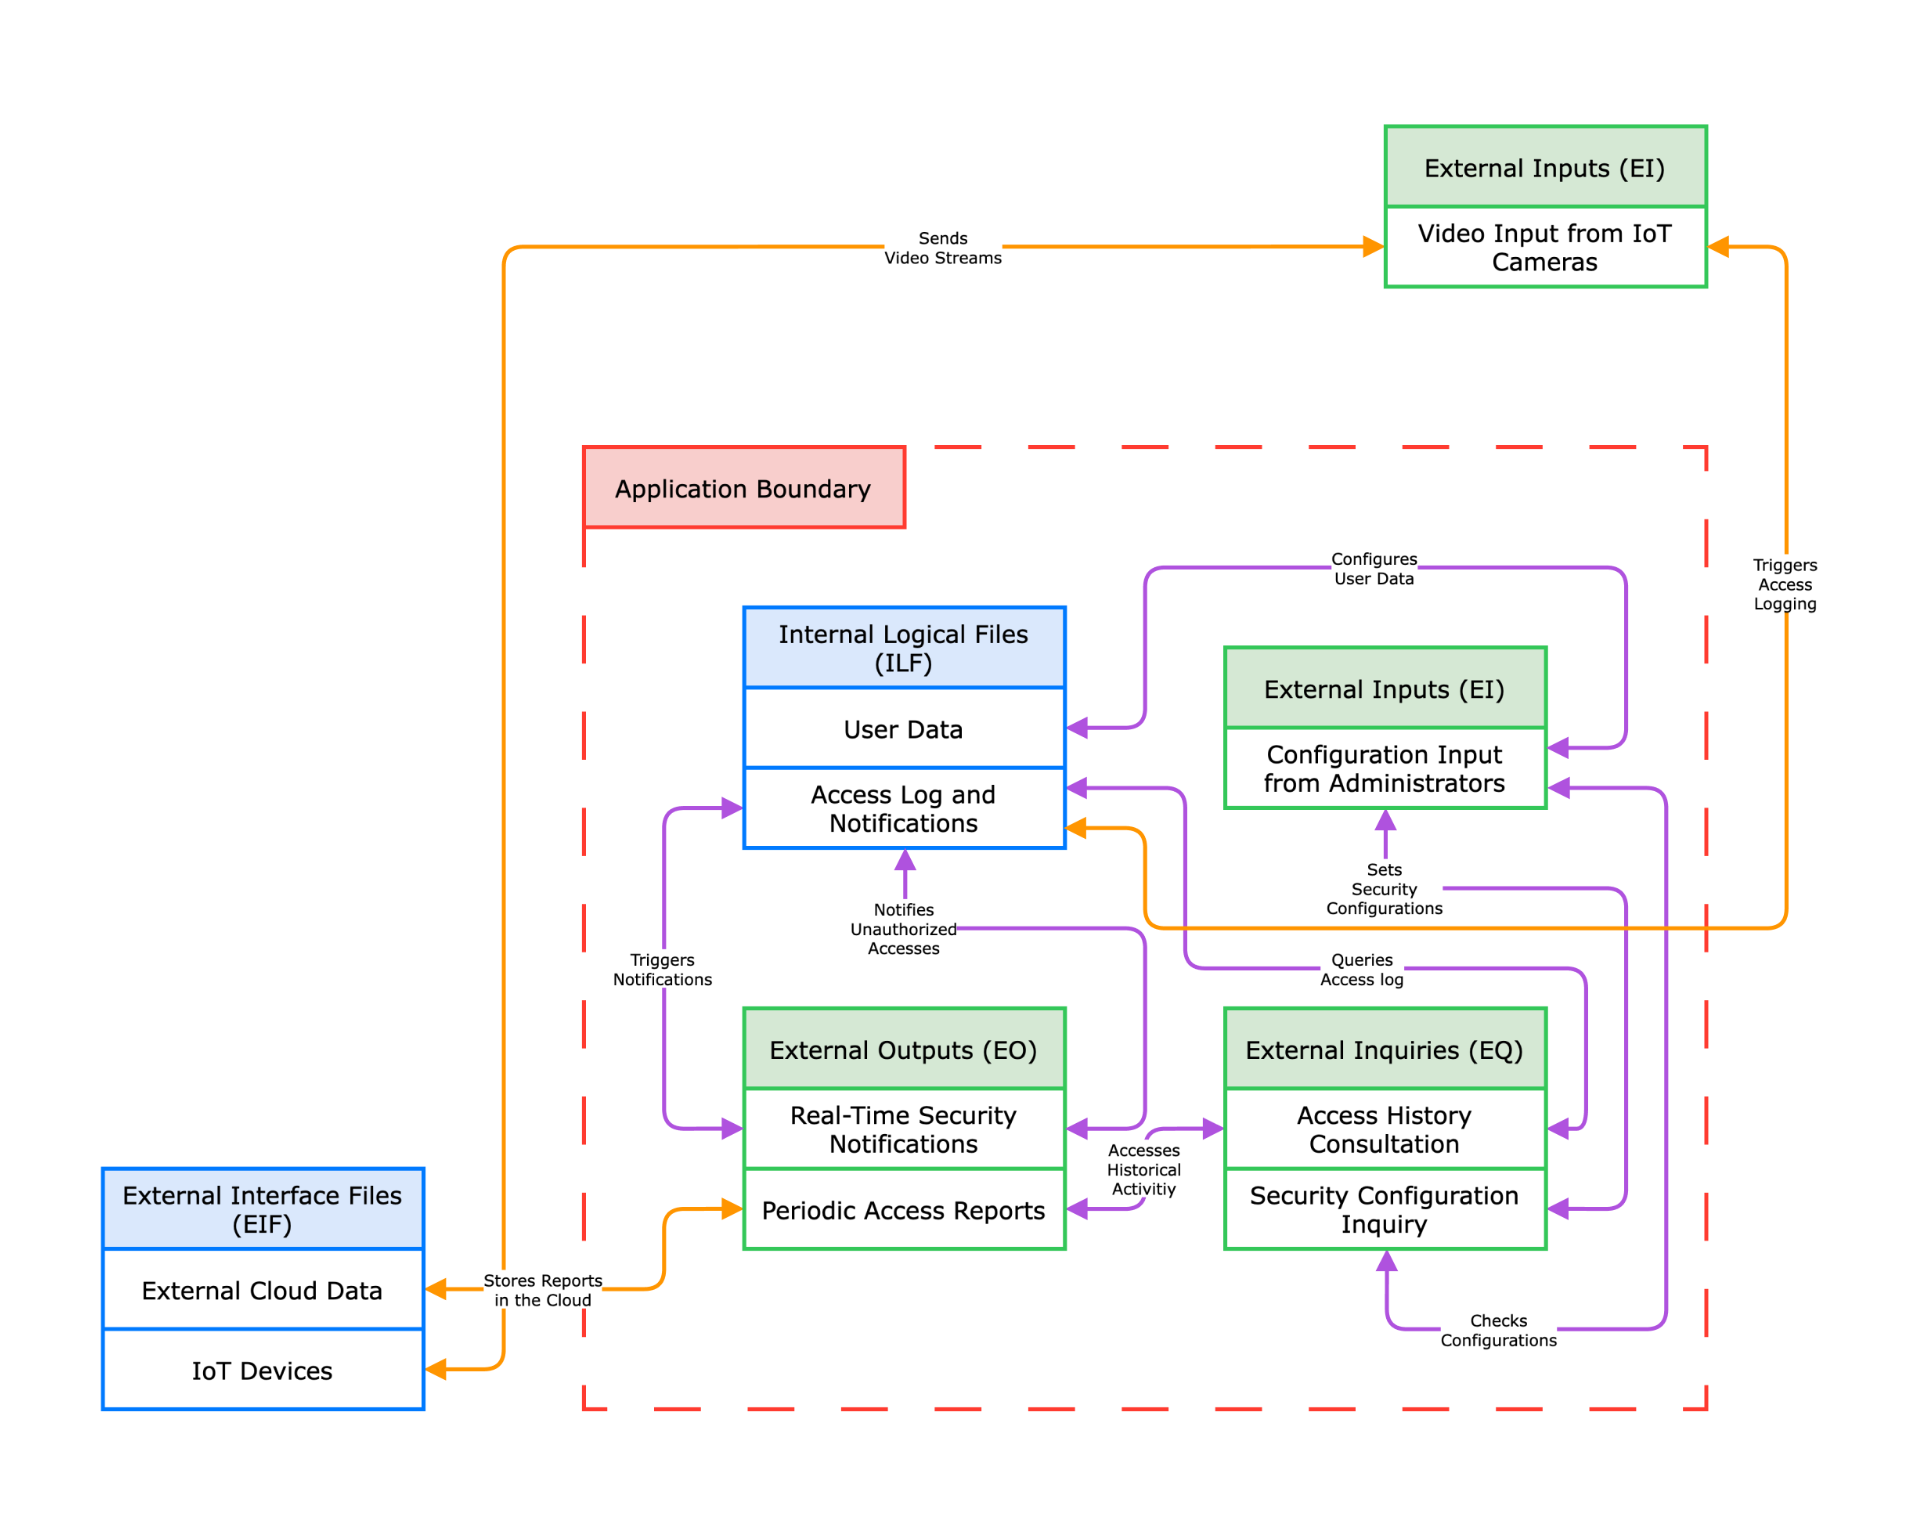
\includegraphics[width=0.7\linewidth]{img/1/1.png}}
    \caption{The diagram shows data flow between the system components.}
    \label{fig:1-1}
\end{figure}
\end{frame}

\begin{frame}[allowframebreaks]{Data Elements Type (DETs)}
\small

\textbf{Internal Logical Files (ILF):}

\begin{itemize}
    \item \textbf{User Data:} Includes ID, name, role, biometric data, access status, etc. (30 DET).
    \item \textbf{Access Log and Notifications:} Access log, timestamp, user ID, action, criticality level, recognition result, notifications, etc. (55 DET).
\end{itemize}

\textbf{External Interface Files (EIF):}

\begin{itemize}
    \item \textbf{External Cloud Data:} Cloud provider configuration data, ID, timestamp, status, fault tolerance, etc. (15 DET).
    \item \textbf{IoT Devices:} IoT device information, ID, type, status, connection, firmware, etc. (20 DET).
\end{itemize}

\framebreak

\textbf{External Inputs (EI):}

\begin{itemize}
    \item \textbf{Video Input from IoT Cameras:} Video feed with metadata: timestamp, camera ID, resolution, etc. (12 DET).
    \item \textbf{Configuration Input from Administrators:} Configuration parameters, ID, security, authorizations, etc. (20 DET).
\end{itemize}

\textbf{External Outputs (EO):}

\begin{itemize}
    \item \textbf{Real-Time Security Notifications:} Content, timestamp, type, level, recipients, etc. (18 DET).
    \item \textbf{Periodic Access Reports:} Access report, violations, timestamp, aggregated details, etc. (25 DET).
\end{itemize}

\framebreak

\textbf{External Inquiries (EQ):}

\begin{itemize}
    \item \textbf{Access History Consultation:} Access history: date, user ID, type, query results, etc. (20 DET).
    \item \textbf{Security Configuration Inquiry:} Displays configuration, ID, security status, access level, etc. (15 DET).
\end{itemize}
\end{frame}

\begin{frame}[allowframebreaks]{Record Elements Type (RETs)}
\small

\begin{itemize}
    \item \textbf{User Data (3 RETs):} User data management includes three distinct categories of data:
    
    \begin{enumerate}
        \item Identification data (e.g., user ID, name, role), used for registration and access management.
        \item Biometric data (e.g., facial data), used for facial recognition.
        \item Access and security data, for traceability and control.
    \end{enumerate}

    \item \textbf{Access Log and Notifications (4 RETs):} This file includes four distinct types of logs:
    \begin{enumerate}
        \item Access log (e.g., timestamp, user ID, access type), to record access activities.
        \item Notification log (e.g., criticality level, notification type), for security notifications.
        \item Violation log (e.g., user ID, unauthorized action), that records unauthorized access.
        \item Change history, to track all administrative actions.
    \end{enumerate}

    \item \textbf{External Cloud Data (2 RETs):} Includes data from various cloud providers to ensure availability and fault tolerance:
    
    \begin{enumerate}
        \item Provider configurations (e.g., provider ID, connection status).
        \item Backup of critical data (e.g., timestamp, backup status) for operational continuity.
    \end{enumerate}

\framebreak

    \item \textbf{IoT Devices (3 RETs):} Gathers information from IoT devices in three distinct categories:
    
    \begin{enumerate}
        \item General device data (e.g., ID, type, status).
        \item Firmware update data (e.g., version, update timestamp).
        \item Connection data and current device status.
    \end{enumerate}
\end{itemize}
\end{frame}

\begin{frame}[allowframebreaks]{File Types Referenced (FTRs)}
\small

\textbf{External Inquiries (EQ):}

\begin{itemize}
    \item \textbf{Video Input from IoT Cameras (2 FTRs):} References the following files to collect and manage camera metadata and monitor access:
    
    \begin{enumerate}
        \item IoT device data to obtain information about recording devices.
        \item Access log and notifications to monitor access and security.
    \end{enumerate}
    
    \item \textbf{Configuration input from administrators (3 FTRs):} Configuration input uses the following files for security configurations:
    
    \begin{enumerate}
        \item Authorized user data to specify roles and authorizations.
        \item Access log and notifications to monitor configuration changes.
        \item IoT device data to update device configurations.
    \end{enumerate}
\end{itemize}

\textbf{External Outputs (EO):}

\begin{itemize}
    \item \textbf{Real-Time Security Notifications (2 FTRs):} References the following files to send notifications based on access events and recipients:
    
    \begin{enumerate}
        \item Access log and notifications to get details of access events.
        \item Authorized user data to identify notification recipients.
    \end{enumerate}
    
    \item \textbf{Periodic Access Report (3 FTRs):} The periodic report accesses the following files to aggregate and present information:
    
    \begin{enumerate}
        \item Access log and notifications for access details.
        \item Authorized user data to link access to users.
        \item IoT device data for information on device access.
    \end{enumerate}
\end{itemize}

\textbf{External Inquiries (EQ):}

\begin{itemize}
    \item \textbf{Access History Consultation (3 FTRs):} Consults the following files to display the complete activity history:
    
    \begin{enumerate}
        \item Access log and notifications for detailed access logs.
        \item Authorized user data to identify the users involved.
        \item IoT device data for information on devices used in access.
    \end{enumerate}

\framebreak

    \item \textbf{Security Configuration Inquiry (2 FTRs):} References the following files to display the current security settings:
    
    \begin{enumerate}
        \item Security parameter configuration for details on current configurations.
        \item Access log and notifications to verify recent configuration changes.
    \end{enumerate}
\end{itemize}
\end{frame}

\begin{frame}[allowframebreaks]{System Complexity}
\tiny

\begin{table}
    \centering
    \begin{tabular}{|l|c|c|c|c|c|}
        \hline
        \textbf{Component}
        & \textbf{Type}
        & \textbf{RETs}
        & \textbf{DETs}
        & \textbf{FTRs}
        & \textbf{Complexity} \\
        \hline
        Authorized User Data
        & ILF
        & 3
        & 30
        & -
        & Average (10) \\
        Access Log and Notifications
        & ILF
        & 4
        & 55
        & -
        & High (15) \\
        Cloud Provider Configurations
        & EIF
        & 2
        & 15
        & -
        & Low (5) \\
        IoT Device Data
        & EIF
        & 3
        & 20
        & -
        & Average (7) \\
        Video Feed for Facial Recognition
        & EI
        & -
        & 12
        & 2
        & Average (4) \\
        Security Parameter Configuration
        & EI
        & -
        & 20
        & 3
        & High (6) \\
        Real-Time Alarm Notifications
        & EO
        & -
        & 18
        & 2
        & Average (5) \\
        Access and Security Report
        & EO
        & -
        & 25
        & 3
        & High (7) \\
        Access History Consultation
        & EQ
        & -
        & 20
        & 3
        & High (6) \\
        Current Security Configurations View
        & EQ
        & -
        & 15
        & 2
        & Average (4) \\
        \hline
    \end{tabular}
    \caption{System complexity calculation.}
    \label{tab:1-1}
\end{table}
\end{frame}

\begin{frame}[allowframebreaks]{Function Points (FPs)}
\scriptsize

\begin{table}
    \centering
    \begin{tabular}{|l|c|c|c|c|}
        \hline
        \textbf{Component}
        & \textbf{Low}
        & \textbf{Average}
        & \textbf{High}
        & \textbf{Total} \\
        \hline
        Input
        & 0 x 3
        & 1 x 4
        & 1 x 6
        & 10 \\
        Output
        & 0 x 4
        & 1 x 5
        & 1 x 7
        & 12 \\
        Inquiry & 0 x 3
        & 1 x 4
        & 1 x 6
        & 10 \\
        ILF
        & 0 x 7
        & 1 x 10
        & 1 x 15
        & 25 \\
        EIF
        & 1 x 5
        & 1 x 7
        & 0 x 10
        & 12 \\
        \hline
        \textbf{FP} &
        & 
        &
        & \textbf{69} \\
        \hline
    \end{tabular}
    \caption{Function Points (FP) calculation.}
    \label{tab:1-2}
\end{table}
\end{frame}

\begin{frame}[allowframebreaks]{Conclusion}
The analysis has provided an overview of the application's structure, focusing on its internal data files, core functionalities, and interactions with external systems.

\bigskip

The system's complexity has been evaluated using function points, revealing a moderate overall complexity score of 69.
\end{frame}

% 
%  BIBLIOGRAPHY 
% 
\begin{frame}[allowframebreaks]{Bibliography}
The analysis was carried out with guidance from the materials of the course \cite{lavazza2024functional}.

\bigskip

\bibliographystyle{plain}
\bibliography{bib/references}
\end{frame}
% 
%  END 
% 

\end{document}